\documentclass[a4paper, 10pt]{scrartcl}

\usepackage[ngerman]{babel}
\usepackage[T1]{fontenc}
\usepackage[utf8]{inputenc}
\usepackage[a4paper,margin=2.5cm]{geometry}
\usepackage{amsmath}
\usepackage{amssymb}
\usepackage{graphicx}

\usepackage[style=science, backend=bibtex]{biblatex} %style=verbose
\bibliography{Theorie_Ultraschall}

\begin{document}
\section{Theorie der zerstörungsfreien Prüfung}
\subsection{Ultraschall-basierte Werkstoffprüfung}
Eines der wichtigsten Verfahren im Bereich der zerstörungsfreien Prüfung ist die Ultraschall-Fehlerprüfung. Es basiert darauf, dass Schallwellen von einem Prüfkopf aus in einen Probekörper eingeleitet und anschließend eventuelle Reflexionen gemessen werden. Diese Messungen werden dann in einem sogenannten Oszillogramm dargestellt.
\begin{figure}[h]\begin{center}
\label{oszillogramme}
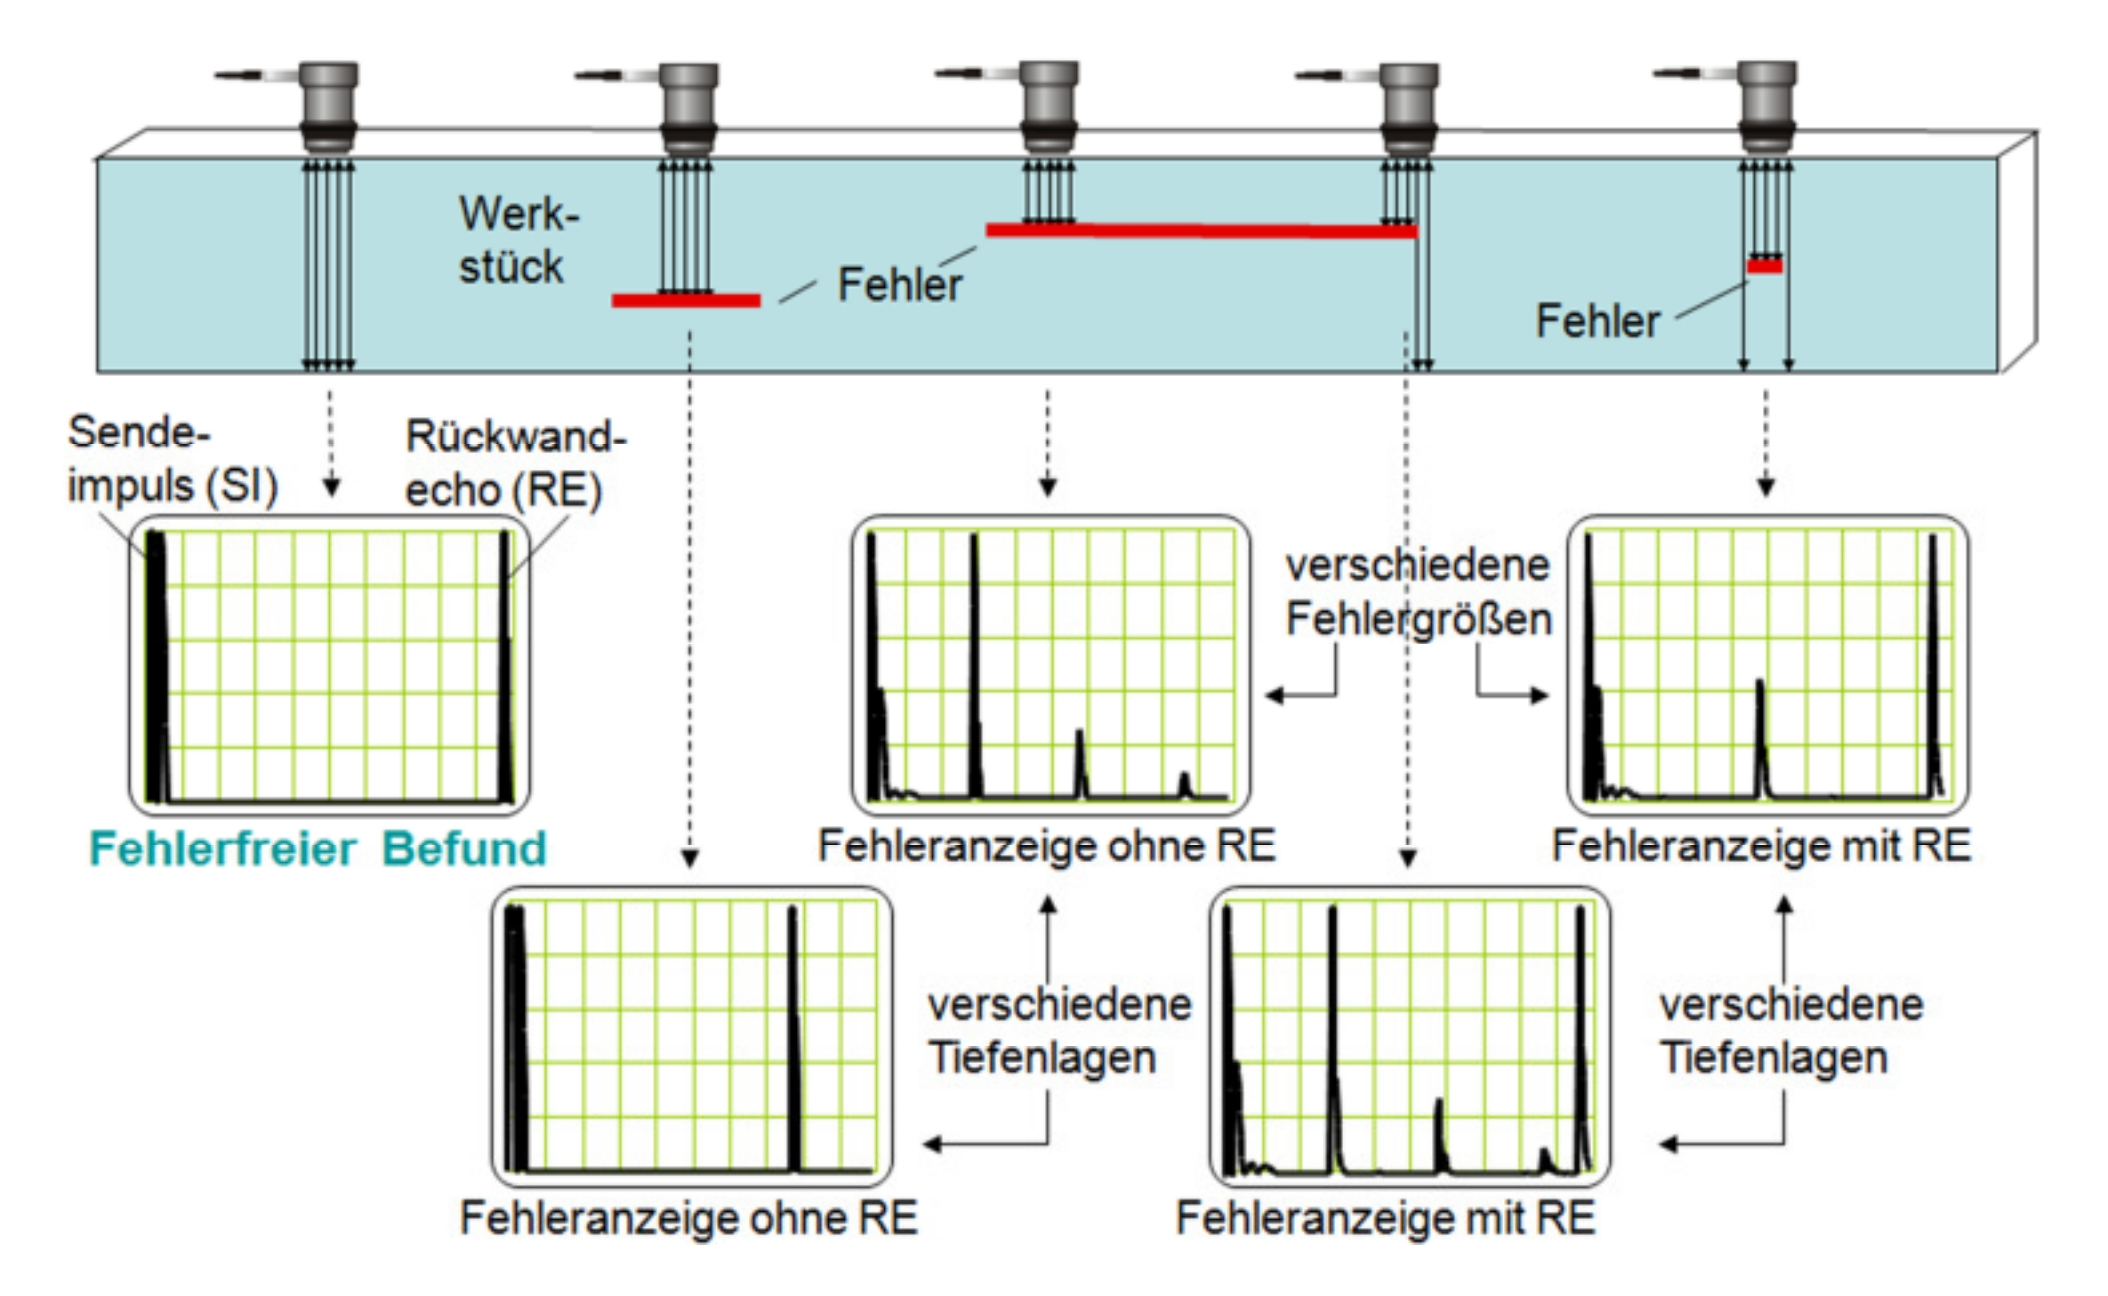
\includegraphics[width=.85\textwidth]{Oszillogramme.jpg}
\caption{Oszillogramme (beispielhaft, Nummer eins bis fünf von links nach rechts)}
\end{center}\end{figure}\\
Je höher dabei eine Spitze (auch Peak) ist, desto stärker war das zugehörige Echo. Hierbei wird ausgenutzt, dass beim Übergang der Ultraschallwellen von einem Material zum anderen ein bestimmter Anteil reflektiert wird, während ein anderer Anteil (unter einem anderen Winkel) sich weiter durch den Körper bewegt. Trifft eine Schallwelle, die sich in einem festen Körper bewegt, auf Luft, so wird sie beinahe vollständig zurückgeworfen, weshalb etwaige passierende Schallwellen gering genug sind, um vernachlässigt werden zu können. So erscheint das erste Echo schon direkt zu Beginn der Messung, wie im ersten Oszillogramm zu sehen: es entsteht, wenn die ausgesandten Wellen in den Probekörper eintreten, denn zwischen Prüfkopf und Probekörper befindet sich immer eine (meist sehr dünne) Luftschicht; daher wird der Schall schon einmal reflektiert, bevor der relevante Teil des Verfahrens beginnt. Um dies in der Praxis zu minimieren, wird eine Kopplungsflüssigkeit verwendet, welche den Schall mit möglichst wenig Reflexionen zwischen Werkstück und Prüfkopf transportiert. Das zweite Echo stellt in diesem Fall das sogenannte Rückwandecho dar, bei welchem die Wellen von der dem Prüfkopf gegenüberliegenden Seite zurückgeworfen werden. Mithilfe dessen kann auch Tiefe des Probekörpers ermittelt werden: da der Schall stets eine materialspezifische Geschwindigkeit $c_\mathrm{Material}$ \cite{schallgeschwindigkeiten} besitzt, gilt für die Stärke des Körpers: $d = \dfrac{c_\mathrm{Material}~\cdot~t}{2}$. Dies ist vor allem hilfreich, wenn Probeköper nur von einer Seite erreichbar sind und ihre Dimensionen daher nicht mit herkömmlichen Werkzeugen bestimmt werden können.\\
Für die zerstörungsfreie Prüfung ist diese Möglichkeit jedoch eher von geringerer Bedeutung. Der eigentliche Nutzen von Ultraschall lässt sich besser an den anderen Oszillogrammen erklären. Befinden sich Fehler im Werkstück, sind das meist Lufteinschlüsse in Form von Rissen oder Löchern. Da sich somit auch dort ein Materialübergang befindet, werden Schallwellen an Fehlstellen ebenfalls reflektiert. Analog zur Bestimmung der Maße des Körpers können auch die ungefähren Positionen der Fehler ermittelt werden. Der große Vorteil dieses Verfahrens ist, dass es nahezu unbegrenzt einsetzbar ist, da sich Sender und Empfänger in einem Gerät befinden und so auch bei komplexen Geometrien, welche nur eingeschränkt zugänglich sind, genutzt werden können. Problematisch ist hingegen die Auswertung der entstehenden Oszillogramme. Zum Beispiel Oszillogramm Nummer vier: einerseits gibt es das normale Rückwandecho, also befindet sich der Prüfkopf teilweise über einem Streifen ohne Fehler; zusätzlich existieren jedoch noch weitere Echos, die auf Fehlstellen hinweisen. Eine mögliche Deutung wäre, dass es mehrere verschieden große Lufteinschlüsse in unterschiedlichen Tiefen gibt, welche die Echos verursachen. Diese Interpretation wäre allerdings falsch, denn wie man sehen kann, gibt es nur einen Fehler, von dem das Echo immer wieder reflektiert wird. An dieser Stelle muss man anmerken, dass in diesem Fall kein gutes Kopplungsmittel verwendet wurde, da sonst das Echo sehr viel schneller abschwächen würde. Der Grund dafür, dass es dennoch schwächer wird, ist einerseits der Fakt, dass die Wellen teilweise die Fehlstelle passieren und somit ein wenig ihrer Stärke verlieren, andererseits aber auch die Streuung der Schallwellen im Körper, sodass das Signal stetig schwächer wird.\\
Im Detail kann die Verfahrensweise der zerstörungsfreien Materialprüfung mit Ultraschall nachgelesen werden in Quelle \cite{karldeutsch}.

\printbibliography
\end{document}